
\chapter{Exporting \pf models as FMUs}
\label{sec:export}

For the purpose of co-simulation it is typically necessary to define a notion of time within a simulation model.
In \pf there are several ways to do so.
In the following, the ways supported by the \fmipp \pf FMU export library are presented.

\subsubsection*{Note:}
Currently only steady-state simulation are supported, where the system's evolution with respect to time comprises a series of load flow snapshots.
RMS simulations are planned to be supported in the future.


\section{Naming convention}
\label{sec:export:naming_convention}

A naming convention is needed that allows to refer to parameters defined in a \pf model in an FMI compliant way (e.g., in the model description).
For the \fmipp \pf FMU export utility this is done by concatenating a parameter's name with the associated object's type and name in the following way:
\begin{verbatim}
FMI compliant name = <object-type>.<object-name>.<parameter-name>
\end{verbatim}
For instance, the parameter \texttt{plini} associated to a general load (object type \texttt{ElmLod}) called \texttt{Load} would be referred to as \texttt{ElmLod.Load.plini} in the model description.


\subsubsection*{Note:}
The naming convention above requires to only use \emph{parameter names} and \emph{object names} that \emph{do not contain periods} "." within \pf models.
Furthermore, the name of objects/parameters has to be \emph{unique within the model}.
These restrictions only apply to objects/parameters that are declared as input or output variables for the co-simulation interface.
It is also recommended to avoid blanks in in the names of such objects/parameters.


\section{Models using external time series and triggers}

\subsection{Creating models using external time series and triggers}

Parameters in \pf can be associated with a time series by providing an external file, called a \emph{Parameter Characteristic from File} (\pf object of type \texttt{ChaVecFile}).
The actual value of the parameter can be changed by associating a user-defined \emph{Trigger and Unit for File} (\pf object of type \texttt{TriFile}) to such a time series.
Figure~\ref{fig:characteristics_from_file} shows the setup window for such a characteristic from file, which defines the associated external file (called \texttt{TestTriggers-characteristics.csv}) and the trigger (defined via the \texttt{Scale} field).
Figure~\ref{fig:trigger_for_file} shows the setup for the trigger itself.
\begin{figure}[h!]
%\vspace*{1em}
\centering{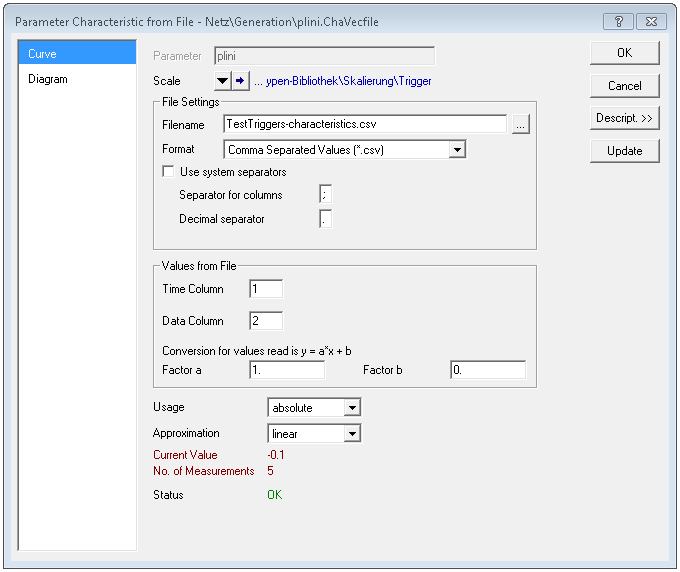
\includegraphics[width=0.9\textwidth]{characteristics_from_file}}
\vspace*{-2mm}
\caption{\pf window for defining a parameter characteristic from file.}
\label{fig:characteristics_from_file}
\vspace*{1em}
\centering{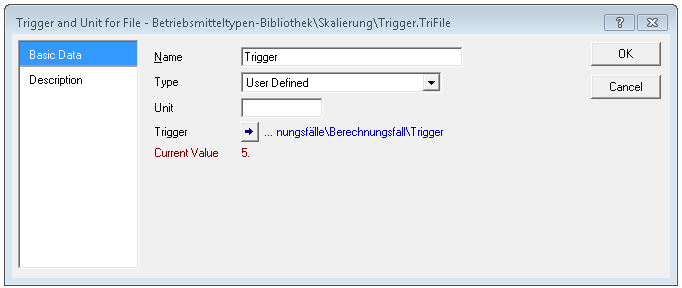
\includegraphics[width=0.85\textwidth]{trigger_for_file}}
\vspace*{-2mm}
\caption{\pf window for defining a trigger and unit for file.}
\label{fig:trigger_for_file}
\end{figure}

%\clearpage

To associate such a time series to a parameter do the following:
\begin{itemize}
  \item select the associated object (double-click)
  \item right-click the input field of the corresponding parameter to bring up the context menu
  \item first select \emph{Add Project Characteristic}, then \emph{Characteristic from File...}
  \item choose the previously created characteristic in the project browser
\end{itemize} 
Figure~\ref{fig:add_characteristics_from_file} shows how the context menus looks like for the example of associating a characteristic from file to the active power parameter of a general load.

\begin{figure}[h!]
\vspace*{2em}
\centering{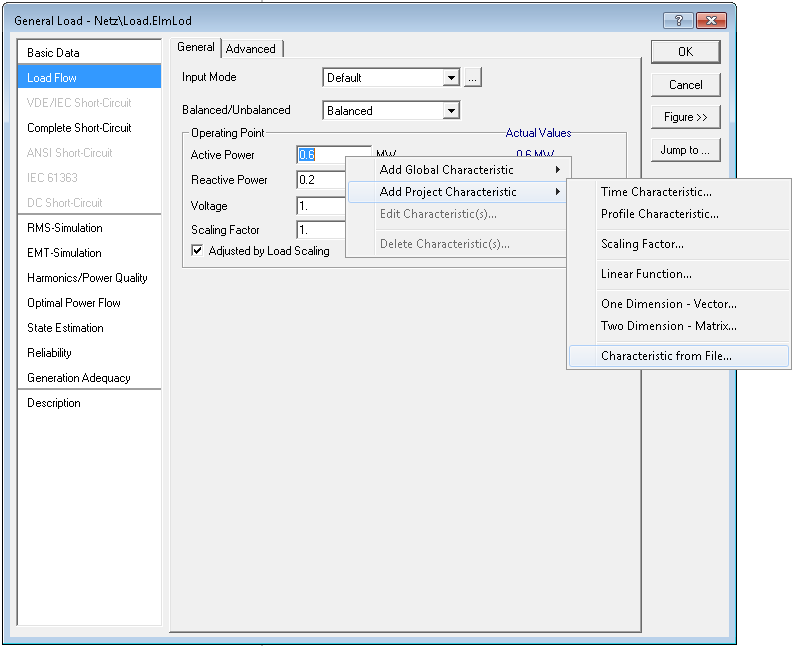
\includegraphics[width=0.9\textwidth]{add_characteristics_from_file}}
\caption{Context menus for associating a time series to a parameter.}
\label{fig:add_characteristics_from_file}
\end{figure}

\clearpage

\subsection{Exporting models using external time series and triggers}

In order to create an FMU from a PFD file that defines characteristics from files and triggers, a \python script has to be executed from the command prompt window (please refer to the \href{https://docs.python.org/2/faq/windows.html}{\python~FAQ} in case you need assistance with this).
Open the command prompt window and execute the script \texttt{powerfactory\_fmu\_create.py}:

\begin{verbatim}
python.exe <path_to_pf_fmu_dir>powerfactory_fmu_create.py [-h] [-v] 
  -m model_id -p pfd_file [-d pf_install_dir] [-i input_var_file]
  [-o output_var_file] [-t name:scale] [additional_file_1 ... ]
  [var1=start_val1 ...]
\end{verbatim}

The path to the \fmipp \pf FMU export utility directory \verb!<path_to_pf_fmu_dir>! may be relative or absolute.
Optional arguments are enclosed by squared brackets \verb![!$\,$\ldots\verb!]!, terms in angle brackets \verb!<!$\,$\ldots\verb!>! represent file paths.
  
\textit{Mandatory input arguments}:
  \begin{itemize}
    \item \verb!-m, --model-id!: specify FMU model identifier
    \item \verb!-p, --pfd-file!: path to PowerFactory PFD file
  \end{itemize}
  \textit{Optional input arguments}:
  \begin{itemize}
    \item \verb!-h, --help!: display the help screen
    \item \verb!-v, --verbose!: turn on log messages
    \item \verb!-l, --litter!: do not clean-up intermediate files
    \item \verb!-i, --input-var-file!: specify file containing list of input variable names
    \item \verb!-o, --output-var-file!: specify file containing list of output variable names
    \item \verb!-t, --trigger!: specify a trigger for advancing simulation time
    \item \verb!-d, --pf-install-dir!: path to \pf installation directory\footnote{It is usually not necessary to provide the path to the \pf installation directory, unless the FMU is intended to run on a another machine with a different installation directory path.}
  \end{itemize}
\end{enumerate}
Files containing lists of input and output variable names are expected to be in clear text, listing exactly one valid variable name per line.
As explained in Section~\ref{sec:export:naming_convention}, variable names are supposed to be of the  form \texttt{<object-type>.<object-name>.<parameter-name>}.

Triggers for simulation time advance need to be defined in the form \texttt{<name>:<scale>}.
The \texttt{name} has to be given according to the trigger's object name in the PFD file.
Times given to the FMU are interpreted as seconds, therefore the \texttt{scale} can be adjusted to match the trigger's internal unit of time (e.g., 60 for minutes or 3600 for hours).
Multiple triggers may be defined.

Additional files may be specified (e.g., CSV load profiles) that will be automatically copied to the FMU. The specified files paths may be absolute or relative.

Furthermore, start values for variables may be defined. For instance, to set a variable with the name \texttt{ElmLod.TestLoad.plini} to a value of 12.34, specify \texttt{ElmLod.TestLoad.plini=12.34} in the command line as optional argument.

Section~\ref{sec:examples:triggers} gives a concrete example of how to export such a model using time series and triggers as an FMU.


\section{Models using a \dplscript to define the time}

\subsection{Creating models using a \dplscript to define the time}
\label{sec:export:create_model_dplscript}

Parameters in \pf can be associated with 1-dimensional vectors, called \emph{Characteristic -- Vector} (\pf object of type \texttt{ChaVec}).
The actual value of the parameter can be changed by associating the elements of such a vector to a \emph{Time Scale} (\pf object of type \texttt{TriTime}) that maps each element to a specific point in time.
Time itself within the model can then be set with the help of a dedicated \dplscript.
Figure~\ref{fig:characteristics_from_vector} shows the setup window for such a vector characteristic, which defines the mapping of the values to the points in time defined by the time scale (defined via the \texttt{Scale} field).
Figure~\ref{fig:trigger_for_vector} shows the setup for the time scale itself.


\begin{figure}[h!]
\vspace*{1em}
\centering{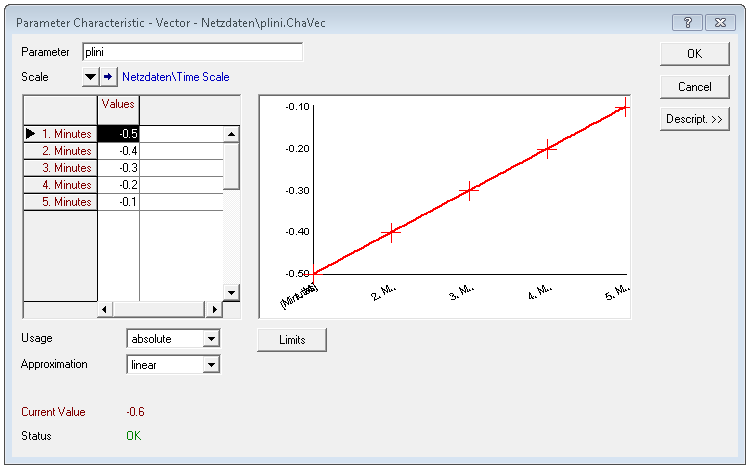
\includegraphics[width=0.9\textwidth]{characteristics_from_vector}}
\caption{\pf window for defining a parameter characteristic from a vector.}
\label{fig:characteristics_from_vector}
\vspace*{2em}
\centering{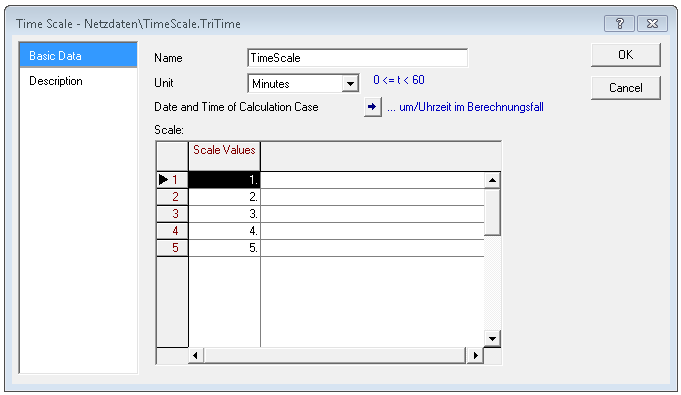
\includegraphics[width=0.85\textwidth]{trigger_for_vector}}
\caption{\pf window for defining a trigger and unit for a vector.}
\label{fig:trigger_for_vector}
\end{figure}

To associate such a vector characteristic to a parameter do the following:
\begin{itemize}
  \item select the associated object (double-click)
  \item right-click the input field of the corresponding parameter to bring up the context menu
  \item first select \emph{Add Project Characteristic}, then \emph{One Dimension -- Vector...}
  \item choose the previously created vector characteristic in the project browser
\end{itemize} 
Figure~\ref{fig:add_characteristic_vector} shows how the context menus looks like for the example of associating a characteristic from file to the active power parameter of a general load.

\begin{figure}[h!]
\vspace*{2em}
\centering{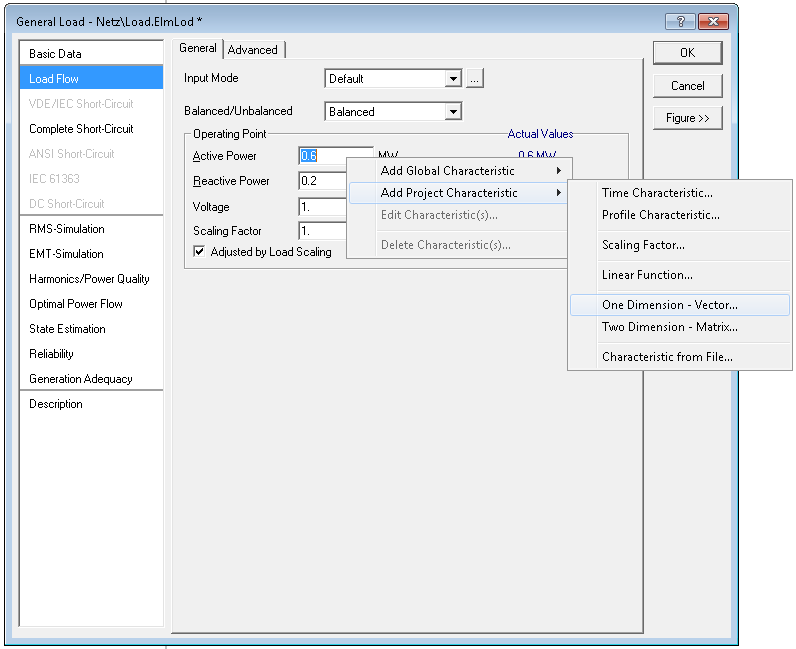
\includegraphics[width=0.9\textwidth]{add_characteristic_vector}}
\caption{Context menus for associating a vector characteristic to a parameter.}
\label{fig:add_characteristic_vector}
\end{figure}

\clearpage

In addition, the \dplscript for setting the time has to be provided.
Such a script could be of the following form:

\begin{Verbatim}[frame=single,commandchars=\\\{\}]

  \codeHighlightGreen{! Change date/time of active study case,}
  \codeHighlightGreen{! using the second of the year as input.}
  \codeHighlightGreen{!}
  \codeHighlightGreen{! ATTENTION: The script doesn't properly}
  \codeHighlightGreen{! handle simulation runs longer than one}
  \codeHighlightGreen{! year.}

  \codeHighlightBlue{object} \textcolor{black}{set_time;}

  \textcolor{black}{set_time =} \codeHighlightBlue{GetCaseObject}\textcolor{black}{(} \codeHighlightRed{'SetTime'} \textcolor{black}{);}

  \codeHighlightBlue{if} \textcolor{black}{( set_time ) \{}
  \textcolor{black}{  set_time:min = 0.0;}
  \textcolor{black}{  set_time:sec = 0.0;}
  \textcolor{black}{  set_time.SetTime( second_of_year * }\codeHighlightDarkRed{0.000277778}\textcolor{black}{ );}
  \textcolor{black}{\}}

\end{Verbatim}
The script's input is the second of the year, represented by variable \texttt{second\_of\_year} (compare to \dplscript setup in Figure~\ref{fig:dpl_script_setup})
The script calculates the hour of the year (by multiplication of $0.000277778 = 1 / 3600$) and and uses this value to set the model's time with the help of function \texttt{SetTime}.
\begin{figure}[h!]
\vspace*{1ex}
\centering{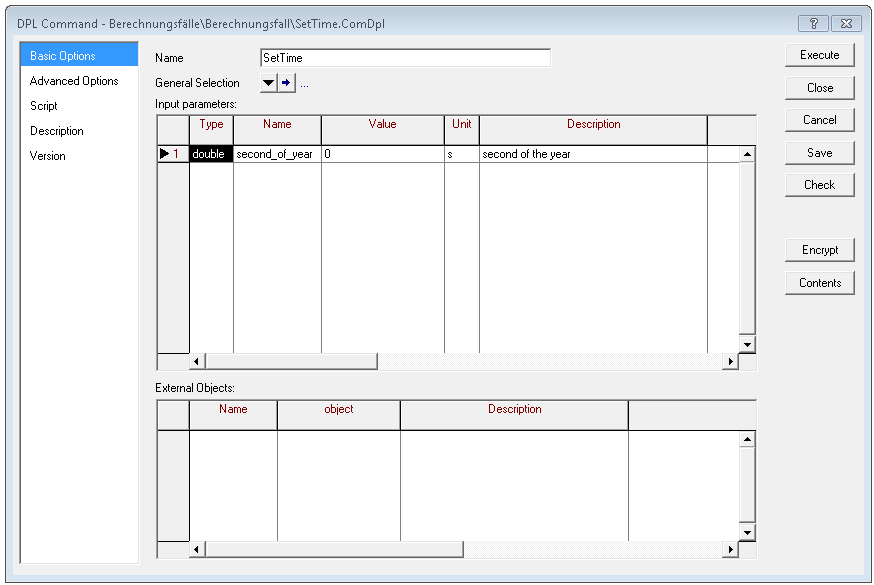
\includegraphics[width=0.95\textwidth]{dpl_script_setup}}
\vspace{-2mm}
\caption{\pf window for \dplscript setup.}
\label{fig:dpl_script_setup}
\end{figure}

\subsection{Exporting models using a \dplscript to define the time}

In order to create an FMU from a PFD file that uses a \dplscript to advance time, a \python script has to be executed from the command prompt window (please refer to the \href{https://docs.python.org/2/faq/windows.html}{\python~FAQ} in case you need assistance with this).
Open the command prompt window and execute the script \texttt{powerfactory\_fmu\_create.py}:

\begin{verbatim}
python.exe <path_to_pf_fmu_dir>powerfactory_fmu_create.py [-h] [-v] 
  -m model_id -p pfd_file [-d pf_install_dir] [-i input_var_file]
  [-o output_var_file] [-s name:scale:offset] [additional_file_1 ... ]
  [var1=start_val1 ...]
\end{verbatim}

The path to the \fmipp \pf FMU export utility directory \verb!<path_to_pf_fmu_dir>! may be relative or absolute.
Optional arguments are enclosed by squared brackets \verb![!$\,$\ldots\verb!]!, terms in angle brackets \verb!<!$\,$\ldots\verb!>! represent file paths.
  
\textit{Mandatory input arguments}:
  \begin{itemize}
    \item \verb!-m, --model-id!: specify FMU model identifier
    \item \verb!-p, --pfd-file!: path to PowerFactory PFD file
  \end{itemize}
  \textit{Optional input arguments}:
  \begin{itemize}
    \item \verb!-h, --help!: display the help screen
    \item \verb!-v, --verbose!: turn on log messages
    \item \verb!-l, --litter!: do not clean-up intermediate files
    \item \verb!-i, --input-var-file!: specify file containing list of input variable names
    \item \verb!-o, --output-var-file!: specify file containing list of output variable names
    \item \verb!-s, --dpl-script!: specify a \dplscript for advancing simulation time
    \item \verb!-d, --pf-install-dir!: path to \pf installation directory\footnote{It is usually not necessary to provide the path to the \pf installation directory, unless the FMU is intended to run on a another machine with a different installation directory path.}
  \end{itemize}
\end{enumerate}
Files containing lists of input and output variable names are expected to be in clear text, listing exactly one valid variable name per line.
As explained in Section~\ref{sec:export:naming_convention}, variable names are supposed to be of the form \texttt{<object-type>.<object-name>.<parameter-name>}.

A single \dplscript may be specified to advance simulation time in the form \texttt{<name>:<scale>:<offset>}.
The \texttt{name} has to be given according to the script's name in the PFD file.
Times given to the FMU are interpreted as seconds, therefore the \texttt{scale} and \texttt{offset} can be adjusted to match the \dplscript's internal representation of time (e.g., 60 for minutes or 3600 for hours).

Additional files may be specified that will be automatically copied to the FMU. The specified files paths may be absolute or relative.

Furthermore, start values for variables may be defined. For instance, to set a variable with the name \texttt{ElmLod.TestLoad.plini} to a value of 12.34, specify \texttt{ElmLod.TestLoad.plini=12.34} in the command line as optional argument.

Section~\ref{sec:examples:dplscript} gives a concrete example of how to export such a model using a \dplscript as an FMU.


\section{Writing additional output}
\label{sec:export:additional_output}

When using a \pf model within a co-simulation, it is possible to write additional simulation results from \pf that are not specified as FMU outputs.
To do so, simply add text files with file extension \texttt{.info} as additional files, containing a list of variable names in clear text, listing exactly one valid variable name per line (just like the input input/output variable name lists for creating an FMU).
For each of these files, a CSV file with the same name (but file extension \texttt{.csv}) will be generated during a simulation run, containing the simulated values of the variables defined in the \texttt{.info} file.
For instance, adding an additional file called \texttt{extra\_data.info} will at simulation time result in the creation of a file called \texttt{extra\_data.csv}.

\subsubsection*{Note:}
These \texttt{.info} files have to be specifically specified as additional files when creating an FMU!